%----------------------------------------------------------------------------
\chapter{Jegyzőkönyv}
%----------------------------------------------------------------------------

%----------------------------------------------------------------------------
\section{Első feladat}
%----------------------------------------------------------------------------
Szelekciós eljárásként a sztochasztikus univerzális mintavételezést kellett megvalósítani. A függvény a pointerek elhelyezése után a Rulettkerék módszerrel választja ki a mintákat. Rekombinációs eljárásként a közbenső, illetve az egyenes mentén történő rekombinációt is megvalósítottuk, a további feladatokhoz az előbbit használtuk.

\lstinputlisting[style=Matlab-editor]{figures/m02/sus.m}\label{SusCode}
\lstinputlisting[style=Matlab-editor]{figures/m02/rws.m}\label{RwsCode}
\newpage
\lstinputlisting[style=Matlab-editor]{figures/m02/recombine.m}\label{XoverCode}

\newpage
%----------------------------------------------------------------------------
\section{Második feladat}
%----------------------------------------------------------------------------
A második feladat során a \textit{genlab} programban található tesztfüggvényeken próbáltuk ki a megvalósított algoritmust. Igyekeztünk a genetikus algoritmus paramétereinek változtatásával a lehető legjobb eredményre törekedni.


A DeJong-függvény esetében a globális és a lokális minimum egybeesik, így itt nem ragadhattunk lokális minimumban, nem megfelelő paraméterezés esetén csupán nem találtuk meg pontosan a függvény minimumát. A további tesztfüggvények viszont több lokális minimummal rendelkeznek, így nem megfelelő paraméterválasztás esetén könnyen lokális minimumban ragadhatunk. A mutáció értékét érdemes viszonylag nagyra választani, mivel így gyakran el tudtuk kerülni a lokális optimumban maradást. A populáció egyedszámát is érdemes nagyra választani (pl. 100 egyed). A legjobb eredményeket a \figref{Dejong}~ábrán szemléltetjük.

\begin{figure}[!h]
	\centering
	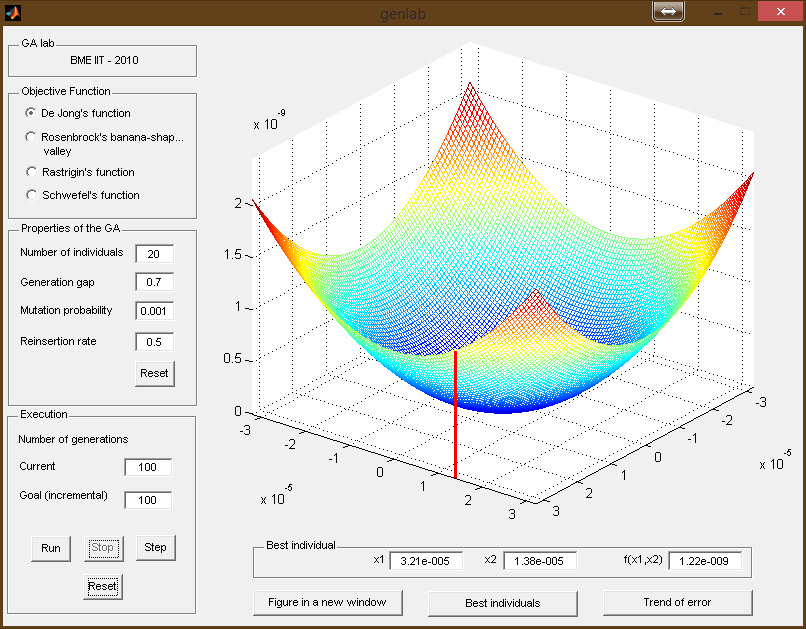
\includegraphics[width=71mm, keepaspectratio]{figures/m02/dejong.png}\hspace{5mm}
	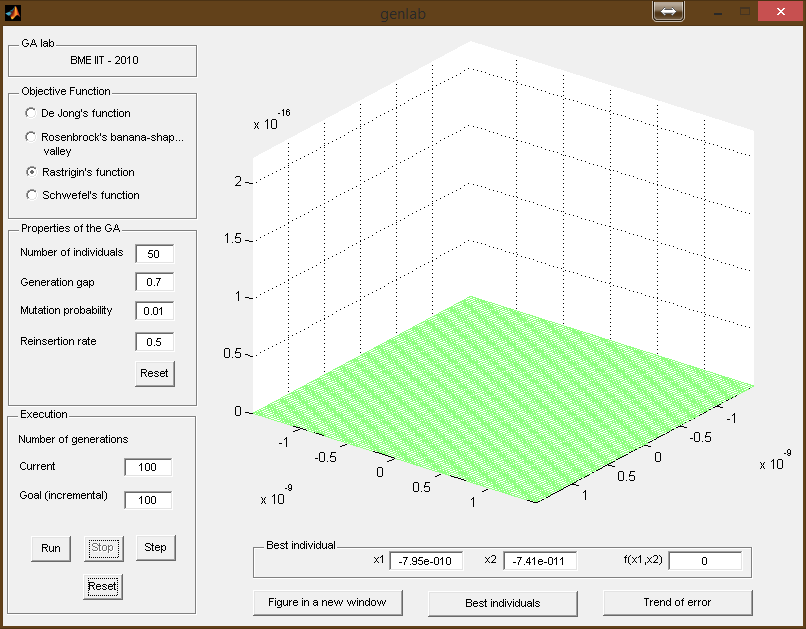
\includegraphics[width=71mm, keepaspectratio]{figures/m02/rastr.png}\vspace{5mm}
	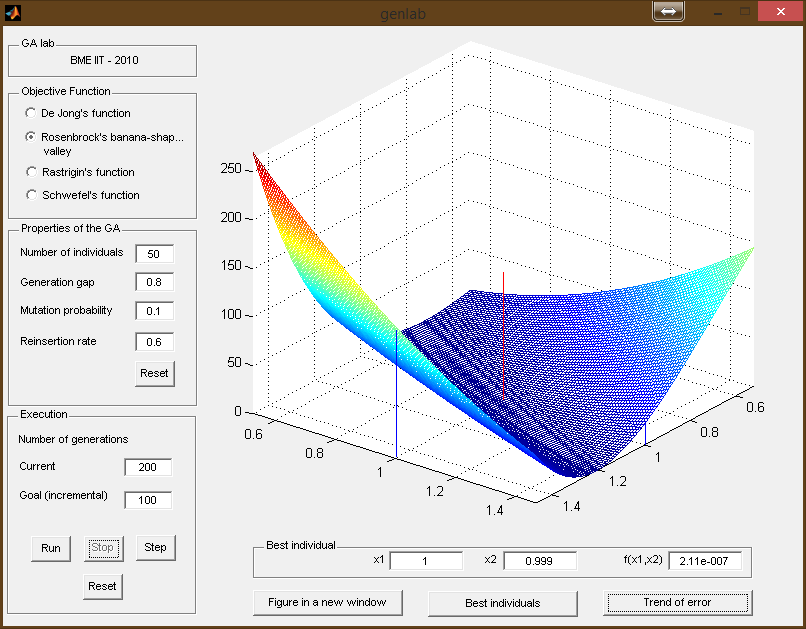
\includegraphics[width=71mm, keepaspectratio]{figures/m02/rosenbr.png}\hspace{5mm}
	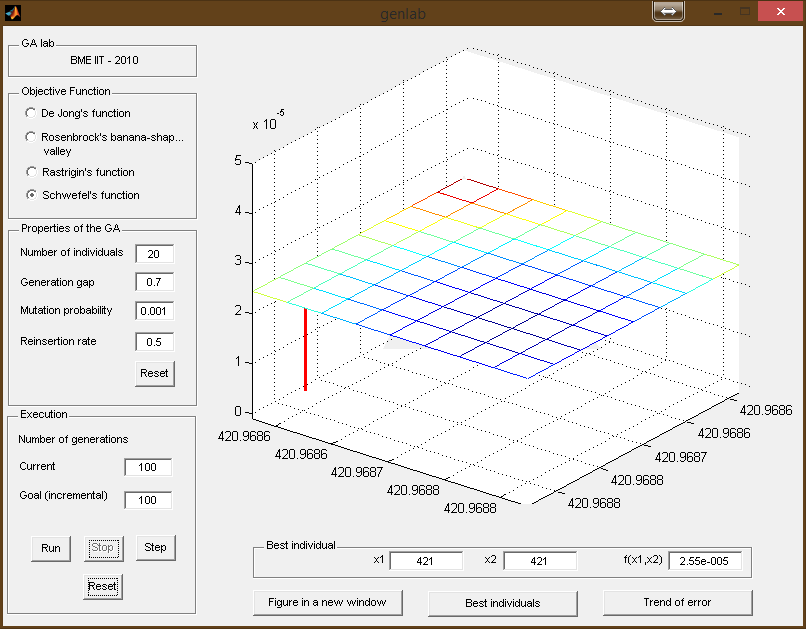
\includegraphics[width=71mm, keepaspectratio]{figures/m02/schwfl.png}
	%TODO ábraelnevezés
	\caption{Tesztfüggvények} 
	\label{fig:Dejong}
\end{figure}

\newpage
%----------------------------------------------------------------------------
\section{Harmadik feladat}
%----------------------------------------------------------------------------
A meghatározott szabályok alapján, a célfüggvény megvalósításához a modellt úgy módosítottuk, hogy kimenetként a szimuláció végén a beavatkozó jel és az alapjel is jelenjen meg, a módosítás a \figref{Control}~ábrán látható.
\begin{figure}[!h]
	\centering
	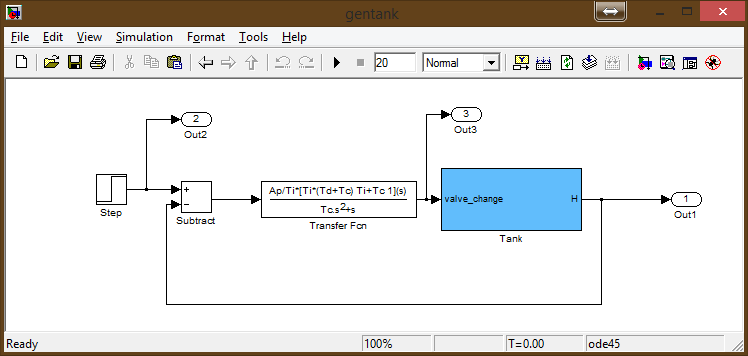
\includegraphics[width=71mm, keepaspectratio]{figures/m02/cntrl.png}
	%TODO ábraelnevezés
	\caption{A módosított modell} 
	\label{fig:Control}
\end{figure}
A költségfüggvényt három hibajel összegeként határoztuk meg. Az első a valódi hibajel integrálja, ez a kimenet és az alapjel különbségéből ered. A másodikként a túllövés miatt keletkezik, itt az 1 érték feletti terület integrálját igyekszünk minimalizálni. Harmadik hibajel a maximálisan kiadható beavatkozó jelből következik. Utóbbi két hibajel súlyozva került bele a költségfüggvénybe, hogy az algoritmus ezeket erősebben optimalizálja.

Számos próbálkozás után a legjobb eredményt egy \textbf{70} egyedből álló populációban találtuk meg, \textbf{100} generáció futtatása után. A szabályzó csupán \textbf{1.21776}-os értékű túllövés mellett, maximálisan \textbf{9.999542}-es beavatkozójelet adott ki \textit{(Paraméterek: Ap=0.909, Td=1.3267, Ti=4.3365, Tc=0.13267)}. Az eredményeket, és a költségfüggvény alakulását a futás során a \figref{PID}~ábrán szemléltetjük, a 
\begin{figure}[!h]
	\centering
	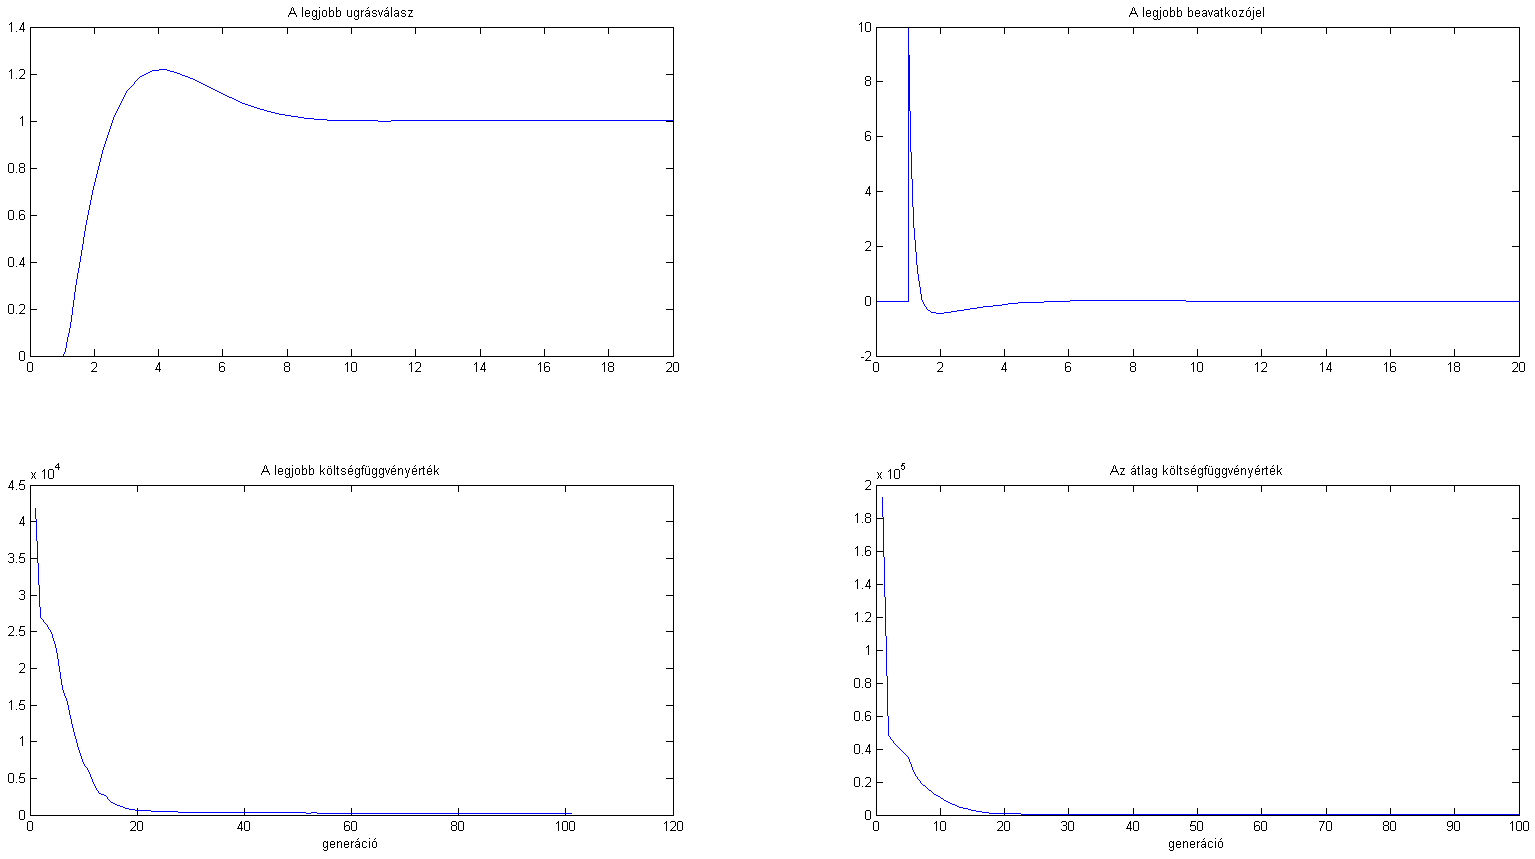
\includegraphics[width=151mm, keepaspectratio]{figures/m02/pid2.png}
	%TODO ábraelnevezés
	\caption{A legjobb eredményt produkáló algoritmus} 
	\label{fig:PID}
\end{figure}
\newpage
\lstinputlisting[style=Matlab-editor]{figures/m02/pid-fctn.m}\label{PidFctn}

%----------------------------------------------------------------------------
\section{Konklúzió}
%----------------------------------------------------------------------------
A genetikus algoritmusok nagyon jól használhatóak optimalizálásra, implementálásuk Matlab környezetben nem túl bonyolult. A futtatásukhoz időre és számítási teljesítményre van szüksége, ám ezek se garantálják a jó eredményt. Az algoritmusok bele tudnak ragadni lokális minimumokba, paraméterezésük időigényes, ám ezzek megfelelő beállítása esetén akár a globális optimumot is képesek megtalálni.


